\graphicspath{{./images/}}

\chapter{Kontextabgrenzung}

\section{Fachlicher Kontext}

\begin{center}
	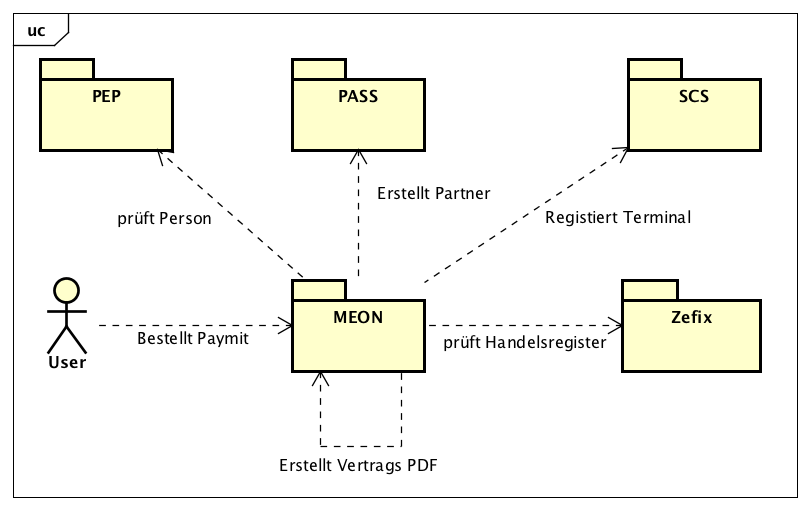
\includegraphics[scale=0.7]{kontext.png}
\end{center}


\section{Technischer Kontext}

Die Applikation MEON basiert auf dem Spring Framework als Backend und AngularJS als Frontent. Die Anwendung wird mittels der Container Technologie Docker ausgerollt. Die Details zum Deployment finden sich im Kapitel Verteilungssicht.

\section{Externe Schnittstellen}

\subsection{PASS Schnittstelle}
		
\subsubsection{Identifikation}

REST Schnittstelle

\subsubsection{Bereitgestellte Resourcen}

- Anlegen eines neuen Partners
- Unblock des Kontos, damit der Partner Zahlungen ausbezahlt bekommt

\subsubsection{Fehlerszenarien}

- Ausfall der Datenbank
- Ausfall Applikationsservers
	
\subsubsection{Variabilitität und Konfigurierbarkeit}

Der Partner wird anhand eines hinterlegten Templates erstellt, nur die davon unterschiedlichen Felder müssen geliefert werden. Die Konfigurierbarkeit ist entsprechend in dem Template, welches über die Schnittstelle mitgegeben wird. Die Schnittstelle ist versioniert für neue Features.
Die URL zeigt auf eine VIP (Virtual IP). D.h. bei einem Ausfall wird (manuell) der Loadbalancer auf den Ausfallserver gerichtet. Da muss die Applikation ebenfalls laufen.

\subsubsection{Qualitätseigenschaften}

Hochverfügbar da über zwei Datenzentern mittels Hot Cold gesichert
Die Schnittstelle nimmt nur zwischen 07:00 und 19:00 Requests an (tagfertige Verarbeitung)
	
\subsubsection{Entwurfsentscheidungen} 

Die Annahme der Request zwischen 7 und 19 Uhr basiert auf dem Modifizerungsmodus für die Benutzer. Theoretisch könnten auch ausserhalb dieser Zeiten neue Partner erstellt werden, da sie das laufende Business nicht beeinflussen. Modifikationen hingegen müssen auf diesen Modus schauen.

\subsubsection{Benutzungshinweise} 

User muss im PASS angelegt sein und die entsprechende Security Role für die Institution beistzen (ist ein technischer, aber auch ein normaler User könnte mit den Berechtigungen das Interface bedienen).
Der Service liegt in der PCI Zone und kann aus der PubDMZ nicht angesprochen werden
	
\subsection{SCS Schnittstelle}

\subsubsection{Identifikation}

\subsubsection{Bereitgestellte Resourcen}

\subsubsection{Fehlerszenarien}

\subsubsection{Variabilitität und Konfigurierbarkeit}

\subsubsection{Qualitätseigenschaften}

\subsubsection{Entwurfsentscheidungen} 

\subsubsection{Benutzungshinweise} 

\subsection{UID Schnittstelle}

\subsubsection{Identifikation}
URL

\subsubsection{Bereitgestellte Resourcen}
Unternehmensdaten

\subsubsection{Fehlerszenarien}
Service nicht verfügbar --> Der User muss von Hand die Daten in der Webapplikation erfassen
Invalide Daten

\subsubsection{Variabilitität und Konfigurierbarkeit}
Histerix

\subsubsection{Qualitätseigenschaften}

\subsubsection{Entwurfsentscheidungen} 

\subsubsection{Benutzungshinweise} 

\subsection{ZEFIX Schnittstelle}

\subsubsection{Identifikation}
URL
\subsubsection{Bereitgestellte Resourcen}
Abfrage Handelsregisterauszug

\subsubsection{Fehlerszenarien}
Unternehmen nicht vorhanden, Handelsregisterauszug muss manuell hochgeladen werden

\subsubsection{Variabilitität und Konfigurierbarkeit}
Kantone haben unterschiedliche Zugangsurls und unterschiedliche Provider
Histerix

\subsubsection{Qualitätseigenschaften}

\subsubsection{Entwurfsentscheidungen} 

\subsubsection{Benutzungshinweise} 

\subsection{Adressen Schnittstelle}

\subsubsection{Identifikation}
URL

\subsubsection{Bereitgestellte Resourcen}
Abfrage Plz/Ort und Strasse

\subsubsection{Fehlerszenarien}
Nicht verfügbar, User muss Adresse ohne Autofill ausfüllen.

\subsubsection{Variabilitität und Konfigurierbarkeit}
Histerix

\subsubsection{Qualitätseigenschaften}

\subsubsection{Entwurfsentscheidungen} 

\subsubsection{Benutzungshinweise} 


